\documentclass[fleqn,usenatbib]{mnras}
\usepackage{amsmath}
\usepackage{graphicx}
\usepackage[T1]{fontenc}
\usepackage{newtxtext,newtxmath}

\DeclareRobustCommand{\VAN}[3]{#2}
\let\VANthebibliography\thebibliography
\def\thebibliography{\DeclareRobustCommand{\VAN}[3]{##3}\VANthebibliography}

\title[Short title, max. 45 characters]{Finding evidence of accreted globular clusters in MW galaxy}

\author[T. Nguyen]{
Toby Nguyen,$^{1}$\thanks{E-mail: publications@ras.ac.uk (KTS)}
Jason Wang,$^{1}$
and Dylan Wenman$^{1}$
\\
$^{1}$School of Physics, University of New South Wales, NSW 2052, Australia\\
}

\date{Accepted XXX. Received YYY; in original form ZZZ}

\pubyear{2024}

\begin{document}
\label{firstpage}
\pagerange{\pageref{firstpage}--\pageref{lastpage}}
\maketitle

\begin{abstract}
In this paper we use data from the Harris catalogue to characterise two subpopulations of globular 
clusters. This analysis is done for the 157 globular clusters found in the Milky way as provided 
by the Harris catalogue however the age-metallicity relation found is only limited to the 55 globular 
clusters examined in the Vandenberg paper. Nevertheless, we find that the Milky Way is home to its 
in-situ population as well as a large group of accreted globular clusters. We suspect that the 
accreted globular clusters come from many different galaxies or satellites but around the same 
time. These accreted globular clusters are bluer in colour, more metal-poor and tend to reside 
further away from the galactic centre than their in-situ counterparts.
\end{abstract}

\begin{keywords}
Globular clusters -- Accreted -- Milky Way -- Kinematics
\end{keywords}

\section{Introduction}

The Milky Way (MW) is home to various star systems, including more than 150 globular clusters.
Globular clusters (GC) are large groups of stars, ranging from ten of thousands to many 
millions members, bound together gravitationally. These GCs orbit around the MW's central 
supermassive blackhole and often reside in the halo of the galaxy. Like other stars who call 
the MW halo as its home, commonly known as Population II stars, GCs tend to be older on average 
compared with other stars in the different components of the MW such as the thin and thick disk \citep{Massari_2019}.
We can look at the spatial distribution and stellar kinematic properties of these GCs to determine 
their formation history. By analysing and grouping their characteristics, we want to be able to 
identify the GCs that are formed within the MW (in-situ) or were accreted from mergers from either 
major or minor galaxies or satellites (ex-situ). From current literature, we understand that the MW 
has not been forming globular clusters for the past $\sim$8 - 10 Gyrs, instead forming all of its 
populations during earlier epochs \citep{belokurov2023insituvsaccretedmilky}.

All massive galaxies contain two populations of GCs, distinct by their colour bimodality of being 
either blue or red \citep{Renaud_2016}. We apply this idea of bimodality in colour to identify two 
subpopulations of GCs in the MW. The bimodality in colour is most likely driven by the bimodality 
in GC metallicity which can be explained in two ways. As GCs form in different epochs, the mechanism 
underlying their formation will be different. For example, for metal-rich stars, these are believed 
to have formed under calm processes of gas accretion and star formation whereas for metal-poor stars, 
they are believed to have formed under turbulent environments, potentially under the impact of mergers 
or interactions \citep{collazos2023galacticarchaeologytracingmilky}.

In this report, we will first analyse the spatial distribution of the MW's GCs. Although we know majority 
of the GC population will sit in the MW halo or thick disk, we expect accreted GCs to be, on average, further 
away from the galactic centre. We will then describe the age-metallicity relation with respect to the GCs, 
outlining the two subpopulations. Finally, the colour and kinematics of the two subpopulations will be studied,
formulating the characteristics and properties of the two red and blue groups. We expect to find that these 
two subpopulations will be distinct in colour and their kinematics \cite{Blom_2014}.

\section{Data}
The Harris catalogue \citep{harris2010newcatalogglobularclusters} contains basic parameters on distances, 
velocities, metalliticies, colors and dynamical parameters for 157 globular clusters in the MW galaxy.
We used spatial data such as galactic radius, $R_{gc}$ as well as a Sun-centered XYZ coordinates system.
The galactic radius of our sun was fixed to be 8 kiloparsecs and so measurements of this kind are relative 
to our sun. The XYZ system uses a cylindrical coordinate system where X points towards the centre of the 
galaxy, Y points in the direction of galactic rotation and Z points towards the galactic North Pole. The 
Harris catalogue also contains information on the colour indicies of the globular clusters. This was 
measured by taking the difference between the flux through different filters, i.e for this report we used 
data from the violet - infrared or $V-I$ filter. Finally, the Harris catalogue contains measures of the 
globular clusters' radial velocity relative to our Sun's neighborhood LSR and central dispersion velocity.
This could be a limiting factor to our analysis on counter-rotators due to the fact that this data would 
not account for our sun's own rotation around the galactic centre. For age data, we turned to the catalogue 
of 55 globular clusters provided by this Vandenberg paper \citep{VandenBerg_2013}. As the 55 globular clusters 
is much less than the 157 globular clusters provided by the Harris data, any plots including age would be 
quite limiting in sample size so any relation involving age would be more indicative rather than conclusive.

\section{Age and metallicity distribution}
We use stellar age to distinguish stars that belong to the MW's different generations. We first plot the 
age and metallicity of all the globular clusters in the MW.

\begin{figure}
    \centering
    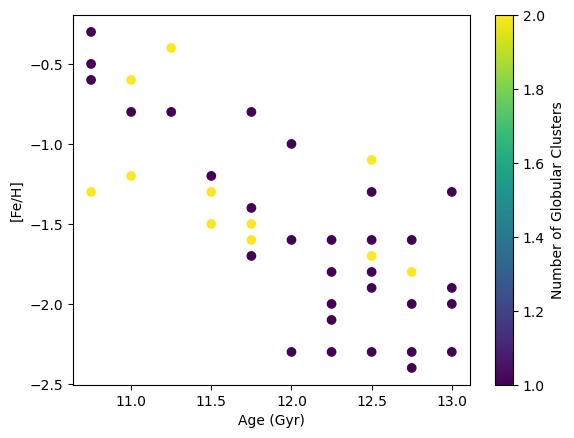
\includegraphics[width=0.32\textwidth]{agefeh.png}
    \caption{Scatter plot displaying the number of globular clusters for a given 
    age and metallicity value. We find that there are two distinct groups in the 
    top left and one subpopulation in the bottom right. These subpopulations 
    include one group that is young but high metallicity and the other being older 
    and less metal rich. We also find at the given ages of 12 to 13 Gyr, there are 
    two subpopulations of higher metallicity and lower metallicity globular 
    clusters.}
    \label{fig:agemetallicity}
\end{figure}

As seen in Figure \ref{fig:agemetallicity}, there is a distinct group of older, less metal rich globular 
clusters. We can argue that this subpopulation represents the accreted globular clusters. Note that the range 
of ages for globular clusters is quite old relative to the rest of the galaxy, i.e 10 to 13 Gyr. This is 
because globular clusters themselves are quite old structures. This means that the accretion event that the 
Milky Way underwent happened relatively early in its lifetime, ending $\sim 1$ Gyr into the Milky way's 
inception. We can infer this because there are no metal poor stars younger than 12 Gyr. The chemical composition 
of the accreted globular clusters indicates that the galaxy of their origin was more metal poor than the Milky 
way.

\section{Spatial distribution of globular clusters}
\begin{figure}
    \centering
    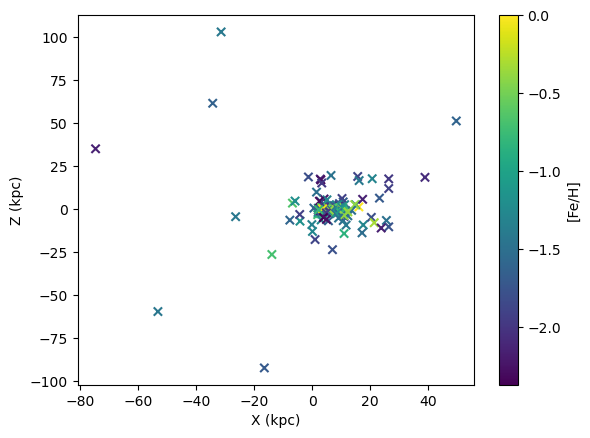
\includegraphics[width=0.35\textwidth]{xzfeh.png}
    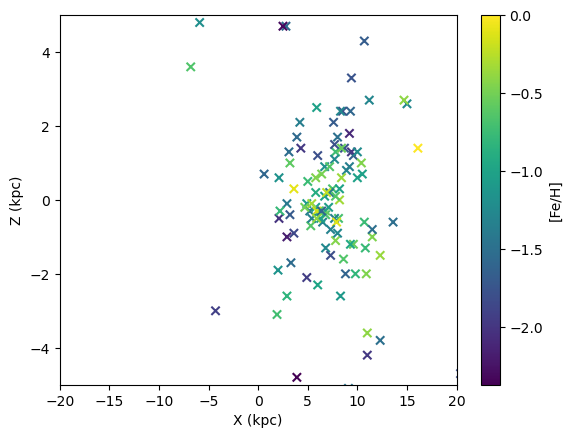
\includegraphics[width=0.35\textwidth]{xzfeh1.png}
    \caption{Top panel: Full zoomed out spatial map of the metallicity of the globular clusters.
    Bottom panel: Zoomed into the cluster of globular clusters in the X = 0 to X = 20 range.}
    \label{fig:xzfeh}
\end{figure}

We can see that in Figure \ref{fig:xzfeh}, lower metallicity globular clusters tend to be in the outer 
regions whilst higher metallicity globular clusters are grouped together tightly. Zooming into the group, 
we can still see this pattern where the higher metallicity globular clusters are in the central regions 
of the group, indicating the distinct subpopulations of the globular clusters are also distinct in their 
position within the Milk Way. The lower metallicity subpopulation residing in the outskirts of the sampled 
data supports this population as being accreted.

\section{Kinematics of globular clusters}
\begin{figure}
    \centering
    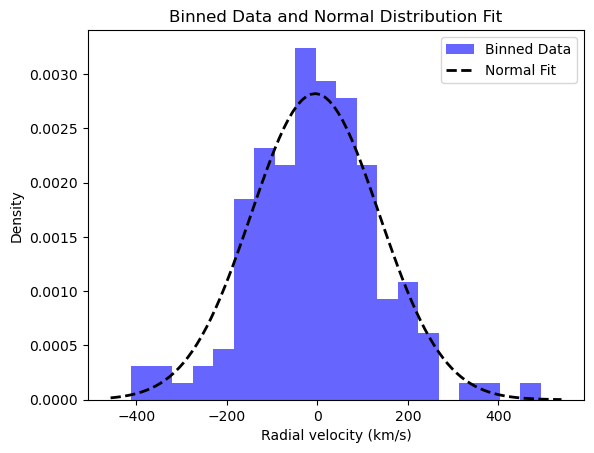
\includegraphics[width=0.23\textwidth]{norm1.png}
    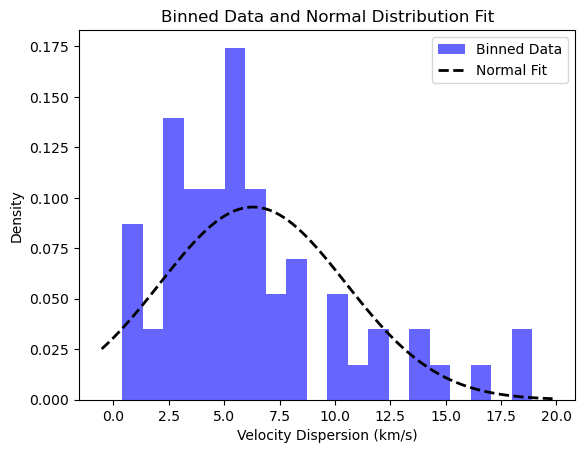
\includegraphics[width=0.23\textwidth]{norm2.png}
    \caption{Left panel: We fitted a Gaussian distribution to the radial velocities provided 
    by the Harris catalogue. The mean is -4.7 km/s and the standard deviation is 141.4 km/s.
    Right panel: We plot the distribution of velocity dispersion of the globular clusters, 
    the mean is 6.3 km/s.}
    \label{fig:norm}
\end{figure}

In Figure \ref{fig:norm}, we find that the radial velocity of the sample is approximately averages out 
to zero, indicating some symmetry amongst the entire population. However if we turn our attention to the 
dispersion velocity distribution, we can see a positive skew. This displays a group of globular clusters 
that are outliers in terms of their dispersive velocity. For old metal poor stars, they have higher 
dispersion velocity compared to their radial velocity \citep{Yu_2017}. Therefore, we can assert that 
these outliers support the hypothesis that the accreted subpopulation of globular clusters are old and 
metal poor.

\begin{figure}
    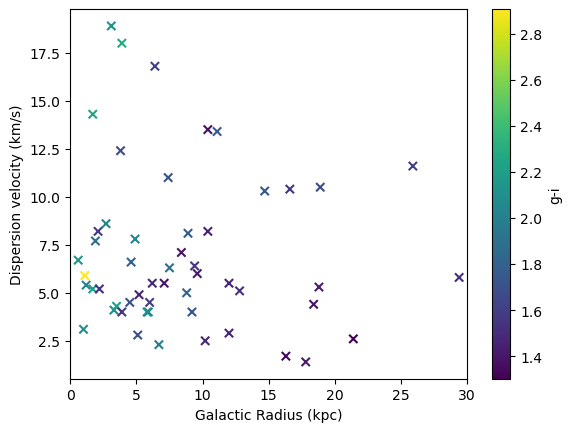
\includegraphics[width=0.35\textwidth]{rgcsigv.png}
    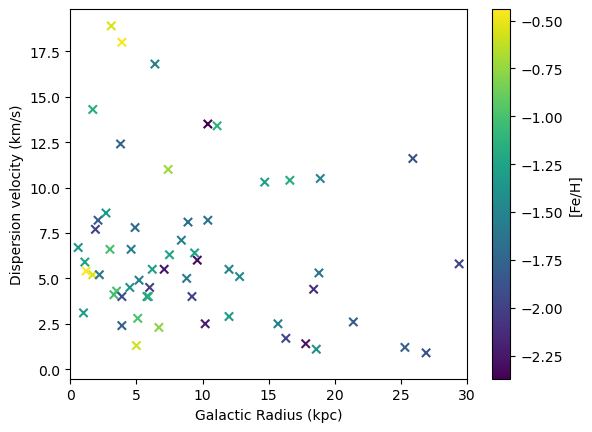
\includegraphics[width=0.35\textwidth]{rgcsigv1.png}
    \caption{Both panels show the dispersion velocity distribution along the galactic radius.
    Left panel: The colour index of each globular cluster is given. Right panel: The metallicity
    of each globular cluster is given.}
    \label{fig:dispersion}
\end{figure}

However, in Figure \ref{fig:dispersion}, we find that these high dispersion velocity globular clusters 
are both redder in colour and more metal rich comparatively, weakening their claims to be accreted. 
Furthermore, we find that the lower dispersion velocity globular clusters are dominated by a more blue 
and more metal poor subpopulation. This indicates dispersion velocity as a weak indicator for accretion. 
This is because since these globular clusters were accreted very early on, their dynamical state is 
essentially the same as their in-situ counterparts. These older stars in the globular clusters would be 
subject to the same interactions with spiral arms or heatings from other satellite galaxies or galaxy 
mergers \citep{Fatheddin_2023}.

\begin{figure}
    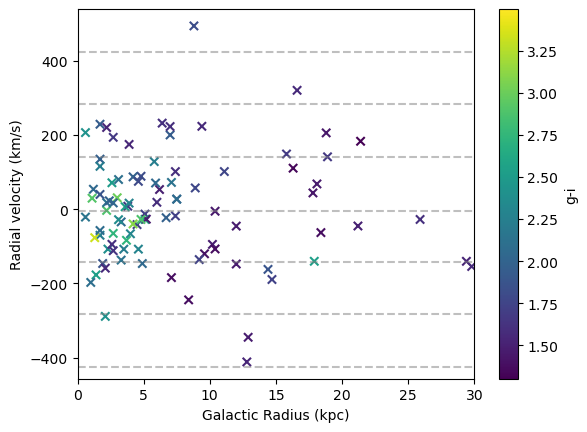
\includegraphics[width=0.35\textwidth]{rgcvr.png}
    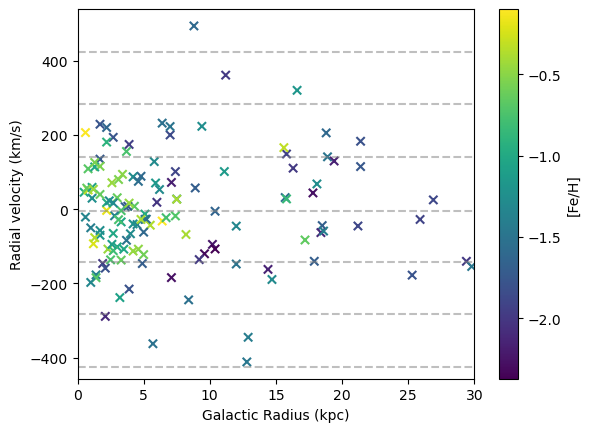
\includegraphics[width=0.35\textwidth]{rgcvr1.png}
    \caption{Both panels show the radial velocity distribution along the galactic radius. Left panel:
    The colour index of each globular cluster is given. Right panel: The metallicity of each globular cluster 
    is given.}
    \label{fig:radial}
\end{figure}

The story is a little bit different in Figure \ref{fig:radial}. We can clearly see two subpopulation 
distinct in their colour and metallicity but now also their radial velocity given their galactic radius.
The red subpopulation has lower radial velocity on average than their blue subpopulation counterparts. 
The red subpopulation ranges from $-1\sigma$ to $1\sigma$ whereas the blue subpopulation spans the whole 
distribution. This is bolstered by looking at the metallicity distribution. We find that the red subpopulation 
is higher in metallicity which indicates they are the in-situ group. 

\section{Discussion}
The Milky Way is host to two large subpopulations of globular clusters. It is likely that the accreted 
subpopulation is blue in colour, more metal poor and exist at a further galactic radius than the in-situ 
globular clusters. The in-situ population is grouped together within the galactic radius of 0 to 10kpc and 
any globular clusters outside of this range is likely to be accreted. The accreted globular clusters have quite 
different kinematic profiles from one another possibly indicating multiple accretion events around the same time 
from different galaxies or the more plausible explanation being that these globular clusters being in different 
points in the Milky Way have undergone different interactions that caused heating, increasing the randomness of 
their motion. This result is largely in agreeance with literature \citep{Gebhardt_1999} whereby cluster galaxies 
such as the Milky Way are always affected by significant accretion, reflected in their host of bimodal globular 
clusters.

Further studies on the the Milky Way globular clusters will need age information for all 157 globular clusters.
Displaying a clear and definitive age-metallicity relation will better distinguish the two subpopulation as well 
as trace the approximate time period of the merger. We also want to improve the kinematic and dynamical analysis 
and so rather than using the Harris catalogue dataset, we should strive to obtain raw LOS data for the entire 
sample. We want to be able to measure the rotational velocity of each globular cluster to better understand their 
kinematics. Finding the Oort constants would also improve our study as then we would be able to find counter-rotators
amongst the globular clusters.

\section{Acknowledgements}
I would like to thank my teammates Dylan and Jason for helping with the research and discussion of ideas for 
this paper. Dr Caroline Foster was instrumental into further developing and assisting in our understanding of 
globular cluster kinematics as well as providing vital feedback in our initial research.

\bibliographystyle{mnras}       
\bibliography{references}         

\label{lastpage}

\end{document}